\documentclass[a4paper, 10pt]{report}

% Packages
\usepackage[italian]{babel}
\usepackage[utf8]{inputenc}
\usepackage[T1]{fontenc}
\usepackage{textcomp}
\usepackage{gensymb}
\usepackage{graphicx}
\usepackage{default}
\usepackage{bbding}
\usepackage{hyperref}
\usepackage{amssymb}


%-----------------------------------------------------------------------
% Documento
%-----------------------------------------------------------------------
\begin{document}
\hypersetup{pageanchor=false}
% Title page
\title{Relazione esercitazione di laboratorio}
\author{Marco Zanella}
\maketitle

\tableofcontents


%-----------------------------------------------------------------------
% Abstract
%-----------------------------------------------------------------------
\begin{abstract}
Il Problema del Commesso Viaggiatore (TSP) è una delle applicazioni più
note del calcolo combinatorio. È classificato come problema \emph{NP-Hard},
per questo motivo risolutori basati su metodi esatti possono impiegare
molto tempo e molte risorse computazionali prima di produrre una soluzione.

In alcuni contesti, il possibile dispendio di tempo e risorse è giustificato
dal vantaggio dato dall'ottenere la soluzione ottima ma, in altre
applicazioni, è preferibile ottenere soluzioni subottime in tempo minore.
Per questo motivo sono state sviluppate euristiche e metaeuristiche per la
risoluzione di molti problemi di natura combinatoria, tra cui il TSP.

In questa relazione sono presentati e messi a confronto un metodo esatto
basato su Programmazione Lineare Intera (PLI) ed un Algoritmo Genetico per
la soluzione del TSP.
\end{abstract}
\hypersetup{pageanchor=true}



%-----------------------------------------------------------------------
% Assunzioni e motivazioni
%-----------------------------------------------------------------------
\chapter{Assunzioni e motivazioni}
\section{Costo degli archi}
\label{sec:assumptions_cost_of_arcs}
Si assume che, dati due nodi, esista al più un arco che porti dal
primo al secondo. Nel caso esistessero più archi possibili, essi
sarebbero noti a priori e la macchina foratrice sceglierebbe comunque
quello meno costoso, riconducendosi allo scenario con al più un
collegamento diretto. La non esistenza di un arco tra due nodi viene
per convenzione rappresentata con una distanza negativa.

Non sono assunte ulteriori proprietà riguardo i costi degli archi: la
matrice dei costi non è necessariamente simmetrica, le distanze non
soddisfano necessariamente la diseguaglianza triangolare e il grafo non
è necessariamente  connesso. Nel caso in cui il grafo non sia connesso,
il problema non ha soluzione.

L'assunzione di non avere un grafo fortemente connesso mira a mettere
in forte difficoltà i risolutori basati su euristiche/metaeuristiche, in
quanto molti degli algoritmi documentati nella letteratura sono in grado di garantire
l'ammissibilità delle soluzioni generate solo a condizione che il grafo
sia fortemente connesso. Non a caso, in letteratura sono poche le fonti
a trattare il TSP su grafi debolmente connessi.

L'assunzione dell'asimmetria ha motivazioni analoghe: è più difficile
lavorare con matrici di distanze asimmetriche. Basti pensare all'esempio
di TSP con Tabù Search visto a lezione: quando si inverte parte di un
cammino (2-opt) nel TSP simmetrico, è possibile aggiornare il costo
della soluzione sottraendo i costi dei due archi rimossi e sommando i
costi dei due archi inseriti. Questo non è più vero quando le distanze sono
asimmetriche: invertendo la direzione degli archi, tutti i costi associati
cambiano ed occorre rivalutare la soluzione (o almeno la porzione
interessata).

L'appendice \ref{app:ideal} mostra un caso di studio semplificato basato
su grafi simmetrici e fortemente connessi.



%-----------------------------------------------------------------------
\section{Ordinamento dei fori}
\label{sec:assumptions_ordering}
Si assume che il nodo da cui cominciare il percorso sia il primo
nodo presente nell'istanza del problema. Tale assunzione non fa perdere
di generalità in quanto la ricerca riguarda un ciclo Hamiltoniano.



%-----------------------------------------------------------------------
\section{Costo della creazione di un modello (CPLEX)}
\label{sec:assumptions_CPLEX}
Si assume che il costo della creazione del modello con CPLEX sia
trascurabile rispetto al tempo di risoluzione. Questa assunzione può
risultare errata per istanze particolarmente piccole ($\approx 5, 10$),
ma si mostra ampliamente corretta per istanze significative. Nel caso di
istanze piccole, inoltre, il tempo globale di esecuzione è comunque
ridotto.

Per questi motivi, e per la sintassi oscura di CPLEX, viene utilizzata una
classe \emph{CPLEXManager} che realizza il \emph{Facade Design Pattern}:
nuove variabili e vincoli vengono aggiunti tramite opportuni metodi, uno
alla volta, tramite un'interfaccia semplificata.
Trattandosi di un \emph{Facade}, non esibisce la stessa
flessibilità della \emph{CPLEX Callable Library} (o di wrapper ufficiali
come \emph{Concert Technology}) ed è ragionevolmente meno efficiente ma,
sotto l'ipotesi del tempo di creazione del modello trascurabile, l'impatto
sul tempo di esecuzione è nullo.



%-----------------------------------------------------------------------
\section{Costo della popolazione iniziale (GA)}
\label{sec:assumptions_GA}
Si assume che il costo per generare una popolazione iniziale per
l'algoritmo genetico si trascurabile rispetto al tempo di risoluzione.
Quest'assunzione è ragionevole poiché i criteri utilizzati nella creazione
della popolazione sono il \emph{Random Walk} ed una semplice euristica
greedy.

Al contrario, essendo il tempo di risoluzione dell'algoritmo genetico
dominante, molte sue componenti sono state scritte in C anziché C++ per
migliorarne l'efficienza (a scapito della semplicità di lettura e
dell'espressività dei linguaggi orientati ad oggetti). Per lo stesso
motivo viene utilizzata la gestione diretta della memoria, anziché
affidarsi ai più dispendiosi meccanismi di C++. Strumenti di analisi
dinamica sono stati utilizzati per testare la corretta gestione della
memoria.



%-----------------------------------------------------------------------
% Modello di PLI
%-----------------------------------------------------------------------
\chapter{Modello di PLI}
Il modello di PLI proposto si basa su quello indicato nella traccia del
progetto.

\section{Rimozione dei cappi}
\label{sec:pli_selfloops}
Poiché nel TSP (così come nel più generale cammino Hamiltoniano) ogni
nodo è visitato una sola volta, gli archi che congiungono un nodo con se
stesso (detti \emph{cappi}) non saranno mai percorsi. Per questo motivo
è ragionevole non inserire nel modello le variabili decisionali che
corrispondono a questi archi. Le variabili decisionali diventano quindi:
\begin{itemize}
  \item $x_{ij}$: numero di unità di flusso trasportate dal nodo $i$ al
        nodo $j$, $\forall (i, j) \in A, i \neq j$
  \item $y_{ij}$: 1 se l'arco $(i, j)$ viene utilizzato, 0 altrimenti,
        \mbox{$\forall (i, j) \in A, i \neq j$}
\end{itemize}
Si osserva che quest'operazione rende il modello più semplice: vengono
introdotte meno variabili e meno vincoli.



%-----------------------------------------------------------------------
\section{Archi mancanti}
\label{sec:pli_missingarcs}
Poiché il grafo non è assunto essere fortemente connesso (sez.
\ref{sec:assumptions_cost_of_arcs}), alcuni archi potrebbero non essere presenti.
Per come è definito il modello (in termini di $A$, l'insieme degli archi),
questo non comporta modifiche. Si osserva tuttavia che il modello viene
reso più semplice in quanto il numero di variabili e vincoli inseriti
è minore od uguale a quello che si avrebbe con un grafo fortemente
connesso.



%-----------------------------------------------------------------------
% Algoritmo Genetico
%-----------------------------------------------------------------------
\chapter{Algoritmo Genetico}

%-----------------------------------------------------------------------
\section{Algoritmo}
L'algoritmo genetico proposto si serve di una ricerca locale per migliorare
i cromosomi che codificano buone soluzioni ed utilizza valori adattivi
per le probabilità di crossover e mutazione \cite[Laoufi et al.]{laoufi}.

\label{sec:ga_algorithm}
\begin{figure}
  \centering
  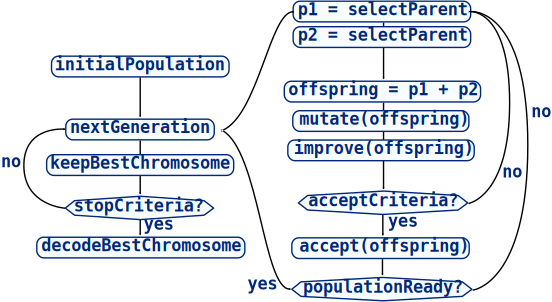
\includegraphics[width=0.95\textwidth]{images/scheme-ga}
  \caption{Schema dell'algoritmo genetico}
  \label{fig:ga_algorithm}
\end{figure}

L'insieme dei cromosomi che codificano soluzioni ammissibili è chiuso
rispetto agli operatori di crossover e mutazione a condizione che il
grafo sia fortemente connesso. Qualora così non fosse, l'approccio
seguito consiste nel penalizzare le soluzioni non accettabili.

La fig. \ref{fig:ga_algorithm} riassume le strategie adottate.



%-----------------------------------------------------------------------
\section{Parametri}
\label{sec:ga_parameters}
L'algoritmo genetico proposto è parametrico rispetto a:
\begin{description}
  \item [pCrossover] Massima probabilità che si verifichi un crossover;
  la probabilità reale è calcolata in maniera adattiva: $p \in [0, pCrossover]$
  
  \item [pMutation] Massima probabilità che si verifichi una mutazione;
  la probabilità reale è calcolata in maniera adattiva: $p \in [0, pMutation]$
  
  \item [threshold] Soglia al di sotto della quale due cromosomi sono
  considerati simili; la distanza di Hamming viene utilizzata come misura
  di somiglianza: $threshold \in [0, 1]$
  
  \item [pAccept] Probabilità di accettare un cromosoma quando ce ne è
  già uno simile presente nella popolazione: $pAccept \in [0, 1]$
  
  \item [pImprove] Probabilità di cercare di migliorare un cromosoma
  considerato \emph{promettente}: $pImprove \in [0, 1]$; un cromosoma è
  \emph{promettente} quando il costo associato alla soluzione da esso
  codificata è inferiore al costo medio della popolazione meno lo scarto
  quadratico medio dei costi
  
  \item [size] Dimensione della popolazione
  
  \item [maxIter] Massimo numero di iterazioni
  
  \item [maxSlack] Numero massimo di iterazioni senza miglioramento;
  permette di identificare convergenze premature
  
  \item [maxTime] Tempo massimo di esecuzione, in secondi
\end{description}

Si osserva come sia sufficiente che uno solo tra \emph{MaxIter},
\emph{maxSlack} e \emph{maxTime} sia verificato per terminare la ricerca.

Dipendere da un elevato numero di parametri è uno svantaggio noto degli
algoritmi genetici. Nell' Appendice \ref{app:calibration} sono spiegate
in dettaglio le tecniche utilizzate per la calibrazione del risolutore.



%-----------------------------------------------------------------------
\section{Componenti}
\label{sec:ga_components}

\subsection{Codifica e decodifica}
La codifica utilizzata è il \emph{Path Representation}: i cromosomi sono
liste di interi, ad ogni intero corrisponde un nodo del grafo. Viene scelta
questa rappresentazione in quanto permette di definire buoni operatori di
crossover e mutazione \cite[Abdoun et al.]{abdoun2012},
\cite[Chatterjee]{chatterjee1996}.

\subsection{Popolazione iniziale}
Gli individui che compongono la popolazione iniziale sono generati
indipendentemente gli uni dagli altri. Ogni individuo è costruito risolvendo
l'istanza del problema con un algoritmo \emph{Random Path} o un'euristica
Greedy (scegliendo non deterministicamente uno dei due approcci).

Il \emph{Random Path} considera una permutazione casuale dei nodi, e la
utilizza come ordine di visita. Il costo computazionale è praticamente nullo,
ma le soluzioni hanno generalmente una bassa qualità (e potrebbero non essere
ammissibili).

L'euristica Greedy parte dal nodo iniziale e si sposta, ad ogni passo, verso
il nodo più vicino non visitato. Il costo computazionale è minimo, ma la qualità
delle soluzioni è poco stabile: per alcune istanze le soluzioni sono molto
buone, per altre sono pessime o non ammissibili. Il problema con questo tipo
di euristica risiede nel fatto che i primi archi scelti hanno costo basso ma,
man mano che l'algoritmo procede, gli archi possibili tendono ad avere costi
più alti.

Questa scelta di generazione della popolazione iniziale è motivata dalla
necessità di avere sia soluzioni il più diverse possibili (quindi è importante
il \emph{Random Path}), sia di introdurre fin dall'inizio delle \emph{buone
caratteristiche}, o \emph{building blocks} (ad esempio grazie all'algoritmo
greedy). È anche importante che la generazione della popolazione iniziale sia
estremamente veloce, a maggior ragione l'uso di permutazioni casuali e greedy
risulta giustificato.


\subsection{Selezione}
La selezione degli individui avviene utilizzando il \emph{Linear Ranking}.
Altre alternative, come \emph{Roulette Wheel} o \emph{Tournament Selection},
producono risultati meno stabili, o funzionano bene solo per istanze relativamente
piccole \cite[Oladele et al.]{oladele2013}, \cite[Noraini et al.]{noraini2011}.

Il \emph{Linear Ranking} opera utilizzando l'informazione sulla posizione in
classifica dei cromosomi, richiede quindi un ordinamento della popolazione ad
ogni iterazione. Si è osservato sperimentalmente che l'overhead dovuto
all'ordinamento è trascurabile.


\subsection{Crossover}
Va osservato che, senza l'assunzione del grafo fortemente connesso,
risulta impossibile definire operatori di crossover e mutazione che
garantiscano risultato ammissibile: le istanze rappresentate da un
grafo sconnesso, ad esempio, non hanno alcuna soluzione ammissibile.
Segue che, comunque siano definiti operatori di crossover e mutazione,
essi non produrranno mai una soluzione ammissibile.

L'approccio proposto consiste nell'utilizzare comunque operatori \emph{buoni},
ovvero che garantiscono ammissibilità a condizione di avere il grafo fortemente
connesso, andando poi a penalizzare le soluzioni non ammissibili. Questa
scelta è motivata dal fatto che, se il grafo è poco connesso, non ci
sono forti motivazioni per utilizzare un operatore piuttosto di un altro:
qualunque operatore si usi, esiste un modo di costruire un'istanza che
lo sfavorisca. Per contro, tanto più il grafo è connesso, tanto
meglio funzioneranno gli operatori \emph{buoni}.

Viene utilizzato il \emph{1-cut Ordering Crossover} tra due cromosomi.
Dopo aver selezionato i due genitori, essi sono soggetti a crossover con
probabilità
$p = pCrossover \cdot \frac{\sigma_c}{c_w - \overline{c}} \in [0, pCrossover] \subseteq [0, 1]$,
dove $\sigma_c$ rappresenta la deviazione standard dei costi delle soluzioni
ammissibili presenti nella popolazione, $\overline{c}$ il loro costo medio
e $c_w$ il costo della soluzione peggiore nella popolazione \cite[Laoufi et al.]{laoufi}.
Nel caso in cui il crossover non avvenga, il nuovo cromosoma è la copia di
uno dei due genitori.


\subsection{Mutazione}
Valgono le osservazioni del punto precedente.

La mutazione proposta è il \emph{2-opt}, ovvero l'inversione di una
porzione della sequenza del cammino. Questa strategia comporta la
rimozione di due archi, l'aggiunta di due nuovi archi e l'inversione
degli archi nella porzione di cammino interessata. Soluzioni non
ammissibili possono essere generate se:
\begin{itemize}
  \item almeno uno dei due archi da aggiungere non esiste
  \item non esiste l'inverso di un arco della porzione da invertire
\end{itemize}

Come per il crossover, la probabilità di mutazione è data da 
$p = pMutation \cdot \frac{\sigma_c}{c_w - \overline{c}} \in [0, pMutation] \subseteq [0, 1]$.

\begin{figure}
  \centering
  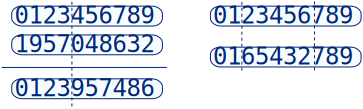
\includegraphics[width=0.95\textwidth]{images/fig-crossover-mutation}
  \caption{Operatori di 1-cut ordering crossover (sinistra) e mutazione 2-opt (destra)}
  \label{fig:crossover-mutation}
\end{figure}


\subsection{Miglioramento}
I cromosomi \emph{promettenti} sono soggetti ad una ulteriore fase di
miglioramento. Un cromosoma $C$ è considerato promettente se
$cost(C) \leq \overline{c} - \sigma_c$, ovvero quando il costo della
soluzione associata è al di sotto della media meno lo scarto quadratico
medio, quindi particolarmente basso.

Poiché il miglioramento comporta comunque un costo computazionale, esso
avviene con probabilità $p = pImprove \in [0, 1]$.

Il miglioramento avviene attraverso una ricerca locale, in particolare
una \emph{Hill Climbing} dove il vicinato è ottenuto considerando le
mosse \emph{2-opt}. È stato scelto questo tipo di ricerca per la sua
velocità e per la qualità dei risultati osservati sperimentalmente
\cite[Ulder et al.]{ulder1991}.


\subsection{Accettazione}
Per mantenere diversificata la popolazione, cromosomi troppo simili
a quelli già presenti non vengono accettati durante la rigenerazione della
popolazione.
La distanza tra due cromosomi $A, B$ è espressa come
$distance(A, B) = \frac{D_H(A, B)}{length(A)} \in [0, 1]$, dove
$D_H(A, B) \in [0, length(A)]$ è la Distanza di Hamming tra $A$ e $B$, e
$length(A) = length(B)$.

Quando si cerca di aggiungere un nuovo cromosoma $o$, se nella
popolazione $\nexists C. distance(o, C) < threshold$, il nuovo cromosoma
viene aggiunto immediatamente. In caso contrario, viene aggiunto con
probabilità $p = pAccept \in [0, 1]$.


\subsection{Gestione della Popolazione}
Viene utilizzata una popolazione a dimensione fissa con \emph{Population
Replacement}.


\subsection{Criteri di arresto}
Il ciclo sulle generazioni si arresta quando risulta verificata almeno
una delle condizioni:
\begin{itemize}
  \item l'algoritmo è in esecuzione da più di $maxTime$ secondi
  \item sono state compiute più di $maxIter$ iterazioni sulle generazioni
  \item nelle ultime $maxSlack$ generazioni non si è avuto alcun miglioramento
\end{itemize}
Il significato delle prime due condizioni è intuitivo. La terza è un
tentativo di identificare una convergenza: se nelle ultime iterazioni
non c'è stato miglioramento, si assume che l'algoritmo stia convergendo.
Questo può essere causato da una convergenza prematura (in tal caso,
probabilmente il risolutore è stato mal configurato), dal raggiungimento
dell'ottimo globale o da una convergenza troppo lenta.



%-----------------------------------------------------------------------
% Analisi dei dati sperimentali
%-----------------------------------------------------------------------
\chapter{Analisi dei dati sperimentali}
\section{Generazione delle istanze}
\label{sec:analysis_instances}
Un'istanza consiste in un grafo pesato di dimensione fissata. La
generazione comprende tre fasi:
\begin{enumerate}
  \item Generazione dei punti
  \item Perturbazione dei punti
  \item Creazione degli archi
\end{enumerate}
Per la prima fase viene utilizzata una distribuzione uniforme sul piano.
La perturbazione altera casualmente le coordinate dei punti usando una
distribuzione normale di media e varianza fissate a priori come parametri.
La creazione degli archi, infine, associa ad ogni arco una distanza utilizzando
l'\emph{Unfair distance}:
$D_u(A, B) = \sqrt[p]{\sum{(|A_x - B_x|^p + |A_y - B_y|^p)}} + \mathcal{N}(\mu, \sigma^2)$.
Se la distanza così ottenuta è superiore ad una data soglia, l'arco non viene
aggiunto.

\begin{figure}
  \centering
  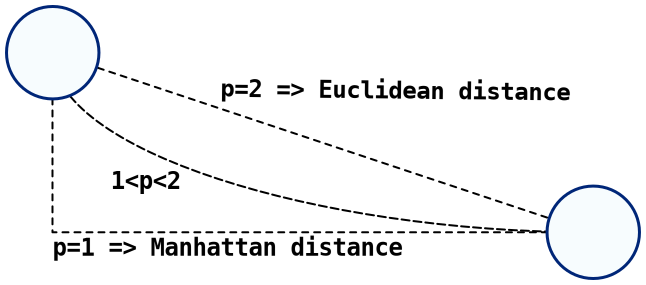
\includegraphics[width=0.95\textwidth]{images/fig-distance}
  \caption{Esempi di Distanza di Minkowski}
  \label{fig:distance}
\end{figure}

Si osserva che il primo addendo altro non è che la \emph{Distanza di Minkowski},
la quale può essere vista come una generalizzazione della \emph{Distanza Euclidea}:
per $p = 2$ si ottiene la distanza Euclidea, per $p = 1$ la distanza Manhattan,
e così via, come esemplificato in fig. \ref{fig:distance}.

Il secondo addendo serve da perturbatore, rendendo la matrice delle
distanze non simmetrica, mentre la soglia permette di scartare
degli archi.

Questo criterio per l'assegnazione delle distanze è giustificato
dall'obiettivo di complicare il problema per un risolutore basato su
euristiche (da cui il nome \emph{Unfair}). Una seconda motivazione è
data dalla descrizione del problema nelle specifiche del progetto:
il costo varia in funzione della macchina foratrice utilizzata. Una
macchina sofisticata, per esempio, è in grado di muoversi
in tutte le direzioni senza vincoli (distanza Euclidea, simmetrica,
fortemente connesso), mentre una macchina meno efficiente potrebbe
essere in grado di spostarsi solo orizzontalmente e verticalmente
(distanza Manhattan), con tempi diversi per gli spostamenti verso
destra o verso sinistra causati da latenze nelle componenti o altri
fattori (matrice asimmetrica), e con un limite alla distanza percorribile
in un singolo passo (grafo non necessariamente fortemente connesso).

\begin{figure}
  \centering
  \includegraphics[width=0.95\textwidth]{images/fig-generator}
  \caption{Esempio di istanza con soluzione ottima evidenziata}
  \label{fig:generator}
\end{figure}

La fig. \ref{fig:generator} mostra un esempio di istanza ottenuta col
procedimento descritto.

Nel codice fornito sono presenti altri metodi per la generazione e
perturbazione di punti, così come altri algoritmi per il calcolo delle
distanze. Questi strumenti sono stati utilizzati in fase di realizzazione
e di test.



%-----------------------------------------------------------------------
\section{Raccolta dei dati}
\label{sec:analysis_gathering}
Al fine di avere un confronto equo tra i due risolutori, ad essi viene
chiesto di risolvere le stesse istanze.

Le statistiche sono prodotte su un insieme di 160 istanze, spaziando
da 10 a 80 nodi per istanza, 20 istanze per ciascuna dimensione. Oltre
ai risultati ottenuti con i risolutori basati su CPLEX ed algoritmo
genetico, vengono mostrati anche quelli ottenuti da un risolutore random,
il quale crea un percorso permutando casualmente l'ordine dei nodi.

Il risolutore random viene introdotto per dare un'idea del guadagno
ottenuto utilizzando una strategia piuttosto che affidarsi ad una
soluzione casuale. Questo tipo di confronto è utile poiché, in alcuni
contesti, risulta più efficiente generare soluzioni casuali molto
velocemente piuttosto che produrne una sola ottima in tempo esponenziale.

\begin{figure}
  \centering
  \includegraphics[width=0.95\textwidth]{images/plot-performance}
  \caption{Qualità delle soluzioni ottenute}
  \label{fig:plot-performance}
\end{figure}

La fig. \ref{fig:plot-performance} mostra le prestazioni ottenute in
funzione della dimensione dell'istanza. Per ciascuna istanza risolta,
la sua prestazione è definita come il rapporto tra il costo della
soluzione ottima ed il costo della soluzione calcolata. La prestazione
mostrata è la media delle prestazioni delle istanze aventi la stessa
dimensione. Poiché CPLEX
produce sempre la soluzione ottima, la sua prestazione è 1. Si osserva
inoltre che, poiché l'algoritmo genetico ha delle componenti casuali,
la prestazione viene calcolata come il costo della soluzione ottima
diviso la media dei costi delle soluzioni calcolate.

Il risolutore random non è stato in grado di generare soluzioni per
nessuna istanza di dimensione 50: tra le permutazioni casuali
considerate, nessuna è risultata ammissibile.

\begin{figure}
  \centering
  \includegraphics[width=0.95\textwidth]{images/plot-wallclock}
  \caption{Tempo di calcolo}
  \label{fig:plot-wallclock}
\end{figure}

La fig. \ref{fig:plot-wallclock} mostra i tempi di esecuzione in funzione
della dimensione delle istanze. Si osservano la crescita esponenziale
del risolutore basato su CPLEX, l'andamento costante del risolutore
random, e la limitazione superiore nel risolutore basato su algoritmo
genetico (dovuta al parametro \emph{maxTime}).

\begin{figure}
  \centering
  \includegraphics[width=0.95\textwidth]{images/plot-cumulative}
  \caption{Percentuale di istanze risolte}
  \label{fig:plot-cumulative}
\end{figure}

La fig. \ref{fig:plot-cumulative} mostra la percentuale (cumulativa) di
istanze risolte entro un dato intervallo di tempo. Si osserva che il
risolutore basato su algoritmo genetico è in grado di risolvere tutte
le istanze entro $\approx 5s$, mentre il risolutore random fallisce
sistematicamente: poiché il grafo non è strettamente connesso, permutazioni
casuali possono produrre sequenze di nodi non connesse da archi.

\begin{figure}
  \centering
  \includegraphics[width=0.95\textwidth]{images/plot-stability}
  \caption{Qualità dell'algoritmo genetico}
  \label{fig:plot-stability}
\end{figure}

La fig. \ref{fig:plot-stability} mostra in dettaglio le prestazioni ottenute
dall'algoritmo genetico in funzione della dimensione dell'istanza,
evidenziando le prestazioni minime e massime registrate e la deviazione
standard dalla prestazione media (le prestazioni sono calcolate con
lo stesso criterio visto per la fig. \ref{fig:plot-performance}).



%-----------------------------------------------------------------------
\section{Confronto}
\label{sec:analysis_comparison}
I risolutori basati su PLI e su GA sono posti a confronto considerando:
\begin{description}
  \item [tempo di sviluppo] misura qualitativa della difficoltà di
  produzione del codice
  
  \item [qualità] quanto le soluzioni sono prossime all'ottimalità
  
  \item [stabilità] tendenza a produrre sistematicamente buone soluzioni
  piuttosto che alcune soluzioni molto buone ma altre pessime
  
  \item [tempo] costo computazionale, tempo di esecuzione
\end{description}

\subsection{Tempo di sviluppo}
I risolutori hanno tempo di sviluppo comparabile. La PLI è generalmente
più difficile da interpretare, ma ben documentata e molti problemi sono
studiati e già tradotti in modelli relativamente semplici da
implementare. Gli algoritmi genetici sono più immediati da comprendere,
e generalmente ben documentati, ma esistono molte varianti e ciascuna
delle componenti può essere implementata con caratteristiche diverse,
rendendo necessari studi e calibrazioni che aumentano il tempo di
sviluppo; d'altro canto, gli algoritmi genetici sono strumenti
totalmente generici, le cui componenti possono essere riutilizzate
facilmente, a differenza dei modelli di PLI.

\subsection{Qualità}
Il risolutore basato su PLI trova sempre la soluzione esatta (quando
questa esiste), ottenendo quindi la massima qualità.

Dalle figg. \ref{fig:plot-performance} e \ref{fig:plot-stability} si osserva come
l'algoritmo genetico proposto abbia una prestazione media superiore all'85\%;
in letteratura non sono presenti sufficienti articoli che trattano grafi
non fortemente connessi per determinare se tale prestazione sia comparabile
allo stato dell'arte o meno, ma resta intuitivamente una prestazione piuttosto
alta. Si osserva inoltre che le prestazioni migliori registrate si mantengono
entro il 5\% dall'ottimo, mentre quelle peggiori promettono prestazioni al di
sopra del 65\%.

\subsection{Stabilità}
Il risolutore basato su PLI è perfettamente stabile, nel senso che
restituisce sempre la soluzioni ottima (quando questa esiste).

L'algoritmo genetico non garantisce di trovare una soluzione, ma nei test
eseguiti è sempre stato in grado di produrne una. La fig. \ref{fig:plot-stability}
mostra inoltre che la qualità media è fortemente spostata verso l'alto, e
la deviazione standard è $< 5\%$: questo significa che le soluzioni
prodotte sono \emph{tendenzialmente} di buona qualità, ed è improbabile
osservare soluzioni significativamente al di sotto della qualità media;
per istanze di dimensione $\leq 50$ è molto probabile ottenere la soluzione ottima,
segue che l'algoritmo genetico proposto mostra una buona stabilità.

\subsection{Tempo}
Il risolutore basato su PLI ha un andamento esponenziale, come era
prevedibile. Va tuttavia osservato che i tempi assoluti sono al di sotto
di un minuto per istanze di dimensione fino a 60, rendendo il problema
gestibile per alcune applicazioni pratiche.

L'algoritmo genetico lavora in tempo costante (grazie all'utilizzo di
\emph{maxTime}). In particolare, nelle simulazioni eseguite, tutte
le istanze sono state risolte in meno di 10 secondi.



%-----------------------------------------------------------------------
% Conclusioni
%-----------------------------------------------------------------------
\chapter{Conclusioni}
\section{Interpretazione}
\label{sec:conclusion_interpeting}
In questa relazione sono stati presentati e messi a confronto due
risolutori per il problema del Commesso Viaggiatore non simmetrico e
non fortemente connesso, uno basato su Programmazione Lineare Intera,
l'altro su Algoritmi Genetici Adattivi con Ricerca Locale.

Entrambi gli approcci hanno permesso di ottenere soluzioni di qualità
significativa ed in tempi ragionevoli. Il risolutore implementato con
CPLEX, in particolare, garantisce l'ottimalità al costo di un moderato
carico computazionale, mentre l'algoritmo genetico lavora in tempo
costante producendo soluzioni vicine all'ottimo.

Non ritengo sia possibile stabilire se uno dei risolutori sia
strettamente migliore dell'altro in quanto, a parità di tempo di sviluppo
e stabilità, uno eccelle nella qualità, l'altro nel tempo di calcolo,
differenze che si fanno tanto più marcate quanto più elevata è la
dimensione delle istanze da risolvere.

Va inoltre osservato che anche altre caratteristiche delle istanze hanno
effetto su qualità e tempo di calcolo: all'aumentare della cardinalità
dell'insieme degli archi nel grafo, aumenta anche il numero di variabili
nel modello lineare, rendendo il calcolo con PLI meno
efficiente, e diminuisce la probabilità di generare soluzioni
inammissibili nell'algoritmo genetico, migliorandone la qualità. Viceversa,
il risolutore basato su PLI è tanto più avvantaggiato quanto più il grafo
è debolmente connesso.

In termini concreti, rispondendo alle specifiche del problema della
macchina foratrice, se il numero di fori è limitato ($\approx 80$) e lo
stesso schema di foratura deve essere rieseguito su più lastre, ritengo
più conveniente utilizzare il modello PLI per calcolare, una sola volta,
i movimenti del trapano da applicare su tutte le lastre. Altrimenti, se il
numero di fori è molto alto, gli scemi di foratura sono troppi e si è
disposti ad accettare un costo subottimo, l'algoritmo genetico è una
buona scelta.



%-----------------------------------------------------------------------
\section{Margini di miglioramento}
\label{sec:conclusion_improvement}
Sarebbe stato positivo introdurre ulteriori criteri per la generazione degli
individui iniziali, ad esempio diversi tipi di greedy o euristiche costruttive
in generale: questo potrebbe introdurre \emph{buone caratteristiche} diverse
che andrebbero ad arricchire la popolazione, migliorando le prestazioni.
Questo miglioramento non è stato realizzato per motivi di tempo.

È noto che la rigenerazione della popolazione può essere resa parallela \cite[Mühlenbein]{muhlenbein1991}.
Tuttavia la programmazione concorrente con pthread è più complessa, richiede
maggiore tempo di sviluppo ed i miglioramenti non sono concettualmente profondi.

Analogamente si possono utilizzare algoritmi genetici distribuiti (ad es. con
MPI) \cite[Braun]{braun1991}, ma anche i questo caso i miglioramenti sono di
tipo architetturale e non concettuale.

Una significativa fonte di miglioramento consiste nello sperimentare diversi
criteri di selezione, crossover, mutation, gestione della popolazione, miglioramento, per
vedere quali danno effettivamente il risultato migliore. Una ricerca esaustiva
richiederebbe però troppo tempo. Sono stati scelti i criteri che, secondo la
letteratura, portano a soluzioni migliori (o comunque quelli meglio documentati).

Il processo di calibrazione può essere ulteriormente raffinato. Due
miglioramenti ovvi sono una ricerca più approfondita nello spazio dei
parametri e la valutazione di modelli diversi oltre al CART. Una miglioria
concettualmente più profonda consiste nel cercare di sfruttare maggiormente
la struttura dell'istanza da risolvere, ad esempio discriminando su quanto
fortemente (o debolmente) il grafo sia connesso.





%-----------------------------------------------------------------------
% Appendici
%-----------------------------------------------------------------------
\appendix
%-----------------------------------------------------------------------
\chapter{Calibrazione dell'Algoritmo Genetico}
\label{app:calibration}
Per la calibrazione dell'algoritmo genetico è stato generato un insieme
di istanze (\emph{calibration set}), distinto rispetto a quello utilizzato
per le statistiche. I parametri rispetto ai quali l'algoritmo è calibrato
sono: $Crossover$, $Mutation$, $Threshold$, $Accept$, $Improve$ e $PopSize$

Idealmente, un test esaustivo deve coprire ogni possibile combinazione
dei parametri. Lo spazio di ricerca esplode quindi in maniera combinatoria.

\begin{figure}
  \centering
  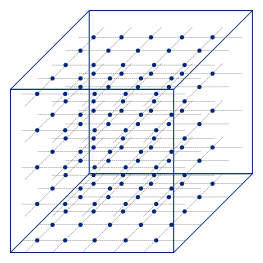
\includegraphics[width=0.45\textwidth]{images/fig-exaustive-training-set}
  \includegraphics[width=0.45\textwidth]{images/fig-reduced-training-set}
  \caption{Calibrazione esaustiva (sinistra) e ridotta (destra)}
  \label{fig:calibration}
\end{figure}

La fig. \ref{fig:calibration} (sinistra) mostra un esempio di spazio di
ricerca esaustivo su tre parametri. Per motivi di tempo non è stato
possibile eseguire la calibrazione esaustiva. Viene quindi proposta una
calibrazione ridotta (esemplificata in fig. \ref{fig:calibration}, destra)
nella quale viene eseguito un numero limitato di test. I valori dei
parametri ad ogni esecuzione sono generati casualmente tramite una
distribuzione uniforme nello spazio di ricerca. Lo spazio delle istanze
diventa così più rarefatto, perdendo tanta più precisione quando più
significativa è la riduzione del numero di test.

Si osserva che, all'aumentare del numero di istanze nella calibrazione
ridotta, questa tende a convergere alla calibrazione esaustiva.

I valori di maxIter, maxSlack, maxTime sono fissati. La calibrazione
è svolta come segue:
\begin{enumerate}
  \item si fissa un insieme di dimensioni di istanze (50, 60, 70, 80)
  \item per ogni dimensione si generano 10 istanze
  \item per ogni istanza, vengono generate 15 configurazioni in maniera
        uniforme
  \item per ogni configurazione, la rispettiva istanza viene risolta 10
        volte con quella configurazione
\end{enumerate}
La ripetizione dell'ultimo punto è necessaria in quanto l'algoritmo
genetico ha alcune componenti casuali.

\begin{table}
  \centering
  \begin{tabular}{|| l | r | l ||}
    \hline
    Parametro   & Coefficiente & Pr(>|t|) \\ \hline
    \hline
    Size        &   -1.707e-03 & < 2e-16  \\
    Crossover   &    1.217e-02 & 0.00692  \\
    Mutation    &    5.294e-02 & < 2e-16  \\
    Threshold   &   -2.943e-02 & 6.77e-12 \\
    Accept      &   -1.774e-02 & 1.22e-05 \\
    Improvement &    5.311e-04 & 0.89831  \\  
    PopSize     &   -8.599e-05 & 0.30942  \\ \hline
  \end{tabular}
  \caption{Influenza marginale dei parametri}
  \label{tab:parameters-marginal}
\end{table}

La calibrazione proposta consiste nello sfruttare l'informazione sulla
dimensione dell'istanza da risolvere per determinare i valori ottimali
dei parametri per l'algoritmo genetico. Dal punto di vista analitico,
si cerca di spiegare la \emph{prestazione} dell'algoritmo su un'istanza
in funzione della dimensione dell'istanza e dei parametri utilizzati. Il
risultato è una relazione che si presenta come funzione
$\mathbb R^5\times \mathbb N^2 \mapsto \mathbb R$, che può essere utilizzata per
determinare quale combinazione di parametri massimizza le prestazioni
(una volta fissata la dimensione dell'istanza).

Per ogni soluzione $i$, la prestazione è calcolata come $\frac{min(c_{istance})}{c_{i}}$,
ovvero il minimo dei costi ottenuti per l'istanza risolta dalla soluzione
$i$ diviso il costo della soluzione $i$ (prestazione relativa).

\section{Effetto marginale dei parametri}
Per avere un'idea dell'effetto marginale dei parametri sulla prestazione,
viene costruito un modello lineare col criterio dei minimi quadrati. La
tab. \ref{tab:parameters-marginal} mostra i coefficienti ottenuti per ciascun
parametro, assieme alla probabilità di osservare un \emph{t-value}
maggiore sotto l'ipotesi nulla. Quest'ultimo dato è una misura della
\emph{significatività} del parametro: quanto più esso è prossimo allo
zero, tanto più la sua influenza sulla performance è significativa.

I parametri $Size, Crossover, Mutation, Threshold$ sono risultati essere
fortemente significativi, mentre $Improvement, PopSize$ sono risultati
scarsamente significativi.

La scarsa significatività di $Improvement$ è motivata dal fatto che
esso è strettamente correlato ad $Accept$, mentre
per $PopSize$ la motivazione risiede nel fatto che la dimensione della
popolazione effettivamente non influenza significativamente la qualità
dell'algoritmo, risultato confermato in letteratura.

Si osserva inoltre
che $Crossover, Mutation, Improvement$ hanno coefficiente positivo:
l'aumento delle probabilità di crossover, mutazione e miglioramento
tramite ricerca locale porta \emph{tendenzialmente} ad un miglioramento
delle prestazioni, come era facilmente intuibile.

Al contrario $Size, Threshold, Accept$
hanno un'influenza negativa: istanze di dimensioni maggiori sono più
difficili da risolvere, soglie molto alte comportano il rifiuto di molti
nuovi individui, ed un'alta probabilità di accettare cromosomi duplicati
comporta scarsa diversificazione nella popolazione.

\section{Distribuzione delle prestazioni}
\begin{figure}
  \centering
  \includegraphics[width=0.45\textwidth]{images/performance}
  \caption{Distribuzione delle prestazioni}
  \label{fig:calibration-performance}
\end{figure}

La fig. \ref{fig:calibration-performance} mostra la distribuzione delle
prestazioni relative durante la calibrazione. Dalla figura si osserva come
i quartili della distribuzione siano spostati verso l'alto. Si osserva
inoltre che la prestazione minima è attorno al $70\%$. Questi risultati
suggeriscono che l'algoritmo proposto è \emph{stabile}, nel senso che
la qualità delle soluzioni fornite si mantiene alta anche in caso di
configurazioni non ottimali, verosimilmente grazie all'utilizzo di
parametri adattivi e della ricerca locale.

\section{Relazione tra parametri e prestazioni}
\begin{figure}
  \centering
  \includegraphics[width=0.95\textwidth]{images/cart}
  \caption{Albero CART}
  \label{fig:calibration-cart}
\end{figure}

La relazione tra i parametri e la prestazione è ottenuta attraverso
l'uso di un CART (\emph{Classification And Regression Tree}).
Idealmente, sono necessari studi preliminari per la scelta
del modello, dei suoi parametri di configurazione, dello spazio
campione e della suddivisione in \emph{training} e \emph{validation set}.
La scelta è stata limitata al CART come strumento \emph{black box}:
la libreria \emph{tree} del software \emph{R} produce un CART
tramite \emph{k-fold cross validation} (suddividendo autonomamente
le istanze in insiemi di allenamento e verifica), e determina
automaticamente i propri parametri di configurazione (come la potatura
dell'albero). La scelta del CART è inoltre motivata dal fatto che
gli alberi prodotti sono più semplici da interpretare rispetto ad
altri modelli (ad es. reti neurali o GAM), e richiedono inoltre un
costo computazionale minimo per essere generati. Gli svantaggi riguardano
il tipo di funzione prodotta (\emph{funzione "a gradini"}),
generalmente meno precisa delle relazioni ricavate da altri modelli,
ed il fatto che un eventuale aggiornamento con nuove osservazioni
comporta il ricalcolo completo del CART stesso. La fig. \ref{fig:calibration-cart}
mostra il CART ottenuto durante la calibrazione.

\section{Funzione di calibrazione}
Sfruttando le informazioni ottenute dal CART e dal modello lineare è
stato creato un risolutore \emph{proxy} che determina i parametri
ottimali in base alla dimensione dell'istanza e richiama il risolutore
genetico proposto. Per determinare i parametri viene utilizzata la
seguente strategia:
\begin{enumerate}
  \item si inizializza un insieme di vincoli $C = \emptyset$
  \item per ogni parametro $p_i$ che rappresenta una probabilità, si
        aggiungono a $C$ i vincoli $p_i \geq 0, p_i \leq 1$; per la
        dimensione della popolazione si aggiunge un vincolo \emph{ragionevole},
        ad esempio $PopSize \geq 16, PopSize \leq 64$
  \item si parte dalla radice dell'albero
  \item se il nodo corrente discrimina sulla dimensione dell'istanza,
        si segue il ramo che corrisponde alla dimensione dell'instanza
        in input (ritorno a 4, considerando il nodo figlio)
  \item se il nodo corrente discrimina su di un parametro, si percorre
        l'arco che porta alla foglia con prestazione più alta, e si
        aggiunge a $C$ il vincolo che soddisfa l'arco scelto (ritorno a 4,
        considerando il nodo figlio)
  \item se il nodo è una foglia, la scansione termina e da $C$ si ottengono
        delle limitazioni inferiori e superiori sui parametri
  \item per ciascun parametro, se il suo coefficiente nel modello lineare è
        positivo viene scelto il suo limite superiore, altrimenti viene
        scelto il suo limite inferiore
\end{enumerate}

Il risultato di questa applicazione è una funzione nella forma
$\mathbb{N} \mapsto \mathbb{R}^5 \times \mathbb{N}$, ovvero una funzione che
data la dimensione di un'istanza, restituisce la configurazione ottimale dei
sei parametri (cinque reali ed uno naturale) dell'algoritmo genetico.



%-----------------------------------------------------------------------
\chapter{Grafo simmetrico e fortemente connesso}
\label{app:ideal}
Nella letteratura il problema del TSP su grafo simmetrico e fortemente
connesso è ampliamente trattato. L'assunzione del grafo fortemente
connesso rappresenta una semplificazione importante sulla natura del
problema, rendendo ogni permutazione una soluzione ammissibile.

Quest'appendice propone un caso di studio su grafi simmetrici e fortemente
connessi, generati con le modalità descritte nella sez. \ref{sec:analysis_instances}.
I grafici presentati sono costruiti in maniera analoga a quelli visti nella
sez. \ref{sec:analysis_gathering}.

In questo caso di studio sono state considerate solo le istanze più \emph{difficili},
quelle aventi dimensioni $60, 70, 80$. Per ciascuna dimensione sono state
generate 5 diverse istanze. Ogni istanza è stata risolta una sola volta col
risolutore basato su PLI, e 10 volte con il risolutore basato su algoritmo
genetico.

\begin{figure}
  \centering
  \includegraphics[width=0.45\textwidth]{images/plot-wallclock-appendix}
  \includegraphics[width=0.45\textwidth]{images/plot-cumulative-appendix}
  \caption{Tempo di calcolo (sinistra) e percentuale di istanze risolte (destra)}
  \label{fig:plot-appendix1}
\end{figure}

\begin{figure}
  \centering
  \includegraphics[width=0.95\textwidth]{images/plot-stability-appendix}
  \caption{Qualità dell'algoritmo genetico}
  \label{fig:plot-appendix2}
\end{figure}

La fig. \ref{fig:plot-appendix1} conferma i risultati presentati nella sez.
\ref{sec:analysis_gathering}: l'algoritmo genetico lavora in tempo
costante, contro il tempo esponenziale impiegato dal modello PLI.

La fig. \ref{fig:plot-appendix2} mostra le prestazioni media, minima e
massima dell'algoritmo genetico, evidenziando la deviazione standard
dalla media. Si osserva che la qualità media delle soluzioni è entro lo
$0.5\%$ dall'ottimo, con la prestazione massima pari a 1. Questo risultato
indica che l'algoritmo genetico è stato in grado di ottenere la soluzione
ottima almeno una volta per ciascuna delle istanze proposte. Si osserva
inoltre che la prestazione peggiore è del $96.5\%$, ovvero che la soluzione
peggiore ottenuta è entro il $3.5\%$ dall'ottimo.

Questi risultati preliminari riguardano un insieme ristretto di istanze,
ma sono incoraggianti in quanto comparabili con lo \emph{stato dell'arte},
nel quale le soluzioni ottenute sono mediamente entro il $3\%$ dall'ottimo:
in \cite[Noraini et al.]{noraini2011}, ad esempio, vengono mostrati
risultati mediamente entro lo $0.9\%$ dall'ottimo, su un insieme di sole
8 istanze.



%-----------------------------------------------------------------------
% Bibliografia
%-----------------------------------------------------------------------
\nocite{nicolas2014}
\bibliographystyle{unsrt}
\bibliography{bibliography}

\end{document}